\chapter{Methodology}
This chapter introduces the reader to the the methodology of the research, investigative work, the subjects under scrutiny and how these leads to the results of this thesis.

\section{International Potential for Free Indoor Mapping Services Survey}
In order to get relevant information regarding the international market for freemium-based \glspl{ims}, and to obtain empirical evidence, a survey was conducted. The survey was done at an international level where respondents were asked to reply to a survey estimated to take between six and eight minutes. The main factor in choosing which \glspl{hei} to contact was the size of the institution, as these might have a larger and inherent need and demand for an \gls{ims}. 


The different institutions were contacted exclusively via email, with the email address and the name of the institution being kept in a spreadsheet to avoid double-contacting people and institutions. Simultaneously this enabled the respective contacts of the survey to be re-contacted. Initially, only the absolute highest ranking official of any given institution was contacted, but consequently the invitation letter was altered slightly, to state that any person with relevant experience may answer the survey. The scope was then widened to include anyone from building- and facilities management, property management, information services management and a larger group of senior officials. Media and communications departments were also contacted, as the invitation letter pleaded recipients to forward the letter to whom it might concern. To follow up non-respondents, each respondent was asked to state their email address and affiliation to avoid being contacted after completing the survey. A new list of non-responders was formed throughout the survey period, and send-outs were performed periodically. Furthermore, they were informed that the survey data was to be handled confidentially, and as such, email addresses and personal information obtained from the survey has purposely been redacted from the thesis. The results can be found as a spreadsheet attachment. The first round of send-outs were conducted in March 2016, and the survey was concluded late June the same year. 

\subsection{Purpose of the Survey}
The primary goal of the survey was to assess and evaluate if customers in the \gls{b2bc}-market would be interested in a freemium-based \gls{ims}. The secondary goal of the survey was to assess the potential customer's willingness to pay for additional services, as this is crucial for the freemium model to be profitable. Additionally, respondents were asked whether or not an \gls{ims} was desirable in the first place. Lastly, a question was raised regarding the potential concerns in the event of a procurement, concerning demand, price and security concerns.

\subsection{Response Rate, Difficulties and Risks}
The main concern when formulating and conducting the survey at an international level, is in many cases the response rate. Given the importance of the empirical data from the survey, this was a concern from the beginning. 


The invitation letter was aptly changed to accommodate for any shortcomings the plan for sending out emails had, to increase the number of respondents. Through an iterative process, the invitation letter was changed so that it was made clear that it was possible to answer the survey in a different way than through Google Forms i.e. via telephone or video conference, but none of the respondents opted for this. Given the low response rate from the initial sendout, telephone calls where considered as means of getting in contact with the correct personnel, but this proved to be time consuming and to little use. During the course of an attempted telephone call, the author would manage to obtain ten or more contacts through email leading to the abandonment of this method of reaching out. From initially only contacting between one and three individuals from an institution, this number was greatly increased through looking up email addresses from the websites of the respective institutions. This tactic increased the response rate from 5\% to over 20\%.  The length of the survey was engineered to be short, as leaders and other senior personnel often have a busy schedule. Additionally, the questions in the survey required little to no knowledge of any technical aspects regarding an indoor mapping solution. This was done in order to appeal to as broad an audience as possible. In total 198 institutions were contacted with 39 answers submitted. A total of 5517 emails were sent, making the average number of emails sent to each institution around 28. 

\newpage

During the first phase of the send-out a script handling sending emails spreadsheet was used. As described above, the spreadsheet contained a column with the numerous email addresses, while another column contained the invitation letter. The last two columns contained information whether the institution had already given an answer or didn't want to be involved with the survey, and the last column contained the name of the institution in order to have a better overview. The scripting language resembles JavaScript, and runs remotely on Google's servers~\cite{google2016} offering its users seamless integration across the various applications and services provided by Google. The source code of the script was inspired by online tutorials, and was customised for the purpose of sending emails using the information in the spreadsheet. The source code of the script can be seen in Listing~\ref{lst:email}. It should be noted that this way of sending out survey invitations was abandoned at a later stage due to inherent limitations in Google's Gmail platform: A limit of 100 recipients per day was simply not enough when the total emails that was due for sending was over 5000. This resulted in abandonment of the script, in favour of using blind copies when sending the huge volume of emails. \gls{ntnu}'s Microsoft Office365 Mail was used instead, as it imposed fewer limitations in the number of emails being sent during a 24-hour period.


The survey itself was conceived and presented in Google Forms, an easy and widespread method not only for making surveys, but also handling replies in the form of a spreadsheet. The invitation letter contained a short URL of a link to the survey. Appendix B shows the survey as presented to the respondents, and Figure~\ref{fig:contactsheet} shows how respondents were being kept track of.

\begin{figure}[H]
    \centering
    \fbox{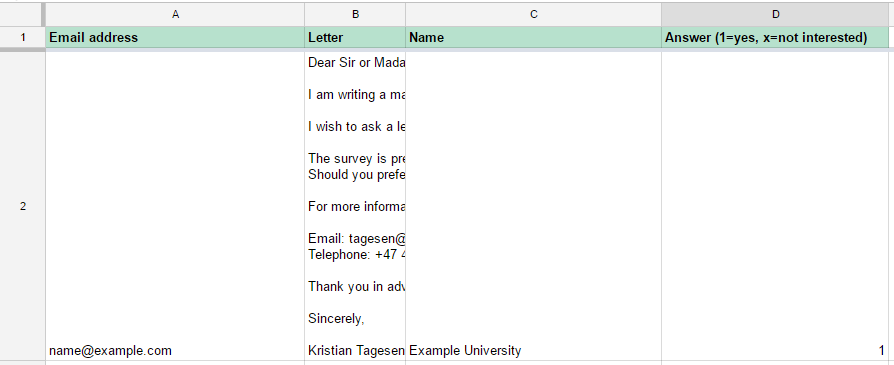
\includegraphics[width=\textwidth]{figs/contactsheet.PNG}}
    \caption{Spreadsheet used to keep track of potential and actual respondents}
    \label{fig:contactsheet}
\end{figure}
\newpage



\lstdefinelanguage{JavaScript}{
  keywords={break, case, catch, continue, debugger, default, delete, do, else, false, finally, for, function, if, in, instanceof, new, null, return, switch, this, throw, true, try, typeof, var, void, while, with},
  morecomment=[l]{//},
  morecomment=[s]{/*}{*/},
  morestring=[b]',
  morestring=[b]",
  ndkeywords={class, export, boolean, throw, implements, import, this},
  keywordstyle=\color{blue}\bfseries,
  ndkeywordstyle=\color{darkgray}\bfseries,
  identifierstyle=\color{black},
  commentstyle=\color{purple}\ttfamily,
  stringstyle=\color{red}\ttfamily,
  sensitive=true
}

\lstset{
   language=JavaScript,
   extendedchars=true,
   basicstyle=\footnotesize\ttfamily,
   showstringspaces=false,
   showspaces=false,
   numbers=left,
   numberstyle=\footnotesize,
   numbersep=9pt,
   tabsize=2,
   breaklines=true,
   showtabs=false,
   captionpos=b
}

\medskip
\begin{lstlisting}[caption=Email Sendout Script,label={lst:email}]
function sendEmails() {
  var sheet = SpreadsheetApp.getActiveSheet();
  var startRow = 2;  // First mail to send
  var numRows = 73;   // Number of emails to send
  // Fetch the range of cells included in this script
  var dataRange = sheet.getRange(startRow, 1, numRows, 2);
  // Fetch values for each row in the Range.
  var data = dataRange.getValues();
  for (i in data) {
    var row = data[i];
    var emailAddress = row[0];  // First column
    var message = row[1];       // Second column
    var subject = "Market potential for free indoor mapping services - MSc Survey";
    GmailApp.sendEmail(emailAddress, subject, message, {from: 'tagesen@stud.ntnu.no', name: 'Kristian Tagesen'});
  }
}
\end{lstlisting}

\section{Business Model Canvas}
A proposed business model is presented in Chapter 6 based on the Business Model Canvas framework, used for mapping existing business models or developing new business models. Originally conceived by Alexander Osterwalder, it is based on his PHd thesis "The Business Model Ontology"~\cite{alexanderosterwalder2004} which eventually lead to the conception of the "Business Model Canvas"~\cite{billmartin2008}. Readers unfamiliar with this concept are referred to Appendix C, where a more detailed introduction to this framework is presented. 